\ifx\allfiles\undefined

	% 如果有这一部分另外的package,在这里加上
	% 没有的话不需要
	
	\begin{document}
\else
\fi

    \chapter{线性规划}
    \section{线性规划问题}
    \subsection{线性规划问题的定义}
    线性规划问题可以归结为\textcolor{red}{求目标函数在约束条件下的最大值问题}。\\
    线性规划模型由以下三个基本要素构成:
    \begin{itemize}[noitemsep]
        \item \textbf{决策变量}:决策变量是问题中要确定的未知量,决策者通过调控决策变量来选取不同的方案、设计、措施以达到最优目的。
        \item \textbf{目标函数}:目标函数通常是决策变量的函数,表达了“何为最优”的准则和目标,规定了优化问题的实际意义。
        \item \textbf{约束条件}:约束条件指决策变量取值 时受到的各种资源和条件的限制,表达了一种“有条件优化”的概念,通常为决策变量的等式或不等式方程。
    \end{itemize}

    \begin{dfnbox}{线性规划问题}{amznotes}
        \dfntxt{线性规划问题} \ 是一类决策变量的取值是\textcolor{red}{连续}的,且目标函数和约束条件都是决策变量的\textcolor{red}{线性函数}的问题
    \end{dfnbox}

    \begin{itemize}[noitemsep]
        \item \textbf{整数规划问题}:决策变量的取值为整数点。
        \item \textbf{混合整数规划问题}:部分决策变量取值连续而其余取值为整数。   
        \item \textbf{非线性规划问题}:目标函数或约束条件中存在任何的非线性因子。
    \end{itemize}

    \subsection{线性规划问题的图解法求解}
    目前,线性规划问题的求解方法主要有两种:
    \begin{itemize}[noitemsep]
        \item \textbf{图解法}:适用于只有两个决策变量的线性规划问题。其可行域可以在平面上画出。
        \item \textbf{单纯形法}:适用于三个决策变量以上数决策变量的线性规划问题。
    \end{itemize}
    \begin{dfnbox}{解的可行域}{amznotes}
        \dfntxt{解的可行域} \ 是满足约束条件的决策变量向量在n维空间中构成的点的集合。
    \end{dfnbox}
    可行域中使得目标函数达到最优的解点成为\textcolor{red}{最优解},相应的目标函数值称为\textcolor{red}{最优值}。
    \\
    \textbf{求解步骤如下}:
    \begin{enumerate}
        \item \textbf{建系}:以两个\textcolor{red}{决策变量}为轴在平面上建立直角坐标系
        \item \textbf{可行域}:由线性等式和不等式构成的\textcolor{red}{约束条件},标出可行域
        \item \textbf{最优解}:图示并移动\textcolor{red}{目标函数},寻找最优解。
    \end{enumerate}
    \begin{exbox}{图解法解线性规划}{coolexample}
        用图解法解下列线性规划:
        \begin{align*}
                \min \; & - x_1 - 4x_2 \\
                \text{s.t.} \quad & x_1 + x_2 \leq 4 \\
                & - x_1 + x_2 \leq 2 \\
                & x_1, x_2 \geq 0
        \end{align*}

        解:
        \begin{enumerate}
            \item 以 ${x}_{1},{x}_{2}$ 为坐标轴画出直角坐标系;
            \item 分别画出 ${x}_{1} + {x}_{2} = 4, - {x}_{1} + {x}_{2} = 2,{x}_{1} = 0,{x}_{2} = 0$ 四条直线,则该问题的可行域为这四条直线包围的内部区域 $\mathrm{s}$ 
            \item 目标函数的等值线方程为 $- {x}_{1} - 4{x}_{2} = z$ 。因为要找的最优解在可行域内使目标函数具有最小值,所以让等值线 $- {x}_{1} - 4{x}_{2} = z$沿 $\mathbf{z}$ 减小的方向在可行域内尽量平行移动,直到图中 ${x}_{1} = 1,{x}_{2} = 3$的位置,如果再移动就移出了可行域 $\mathbf{s}$ 。于是,点(1,3)即为问题的最优解, 目标函数的最优值为 -13。
        \end{enumerate}
    \end{exbox}
    \begin{figure}[H]
        \centering
        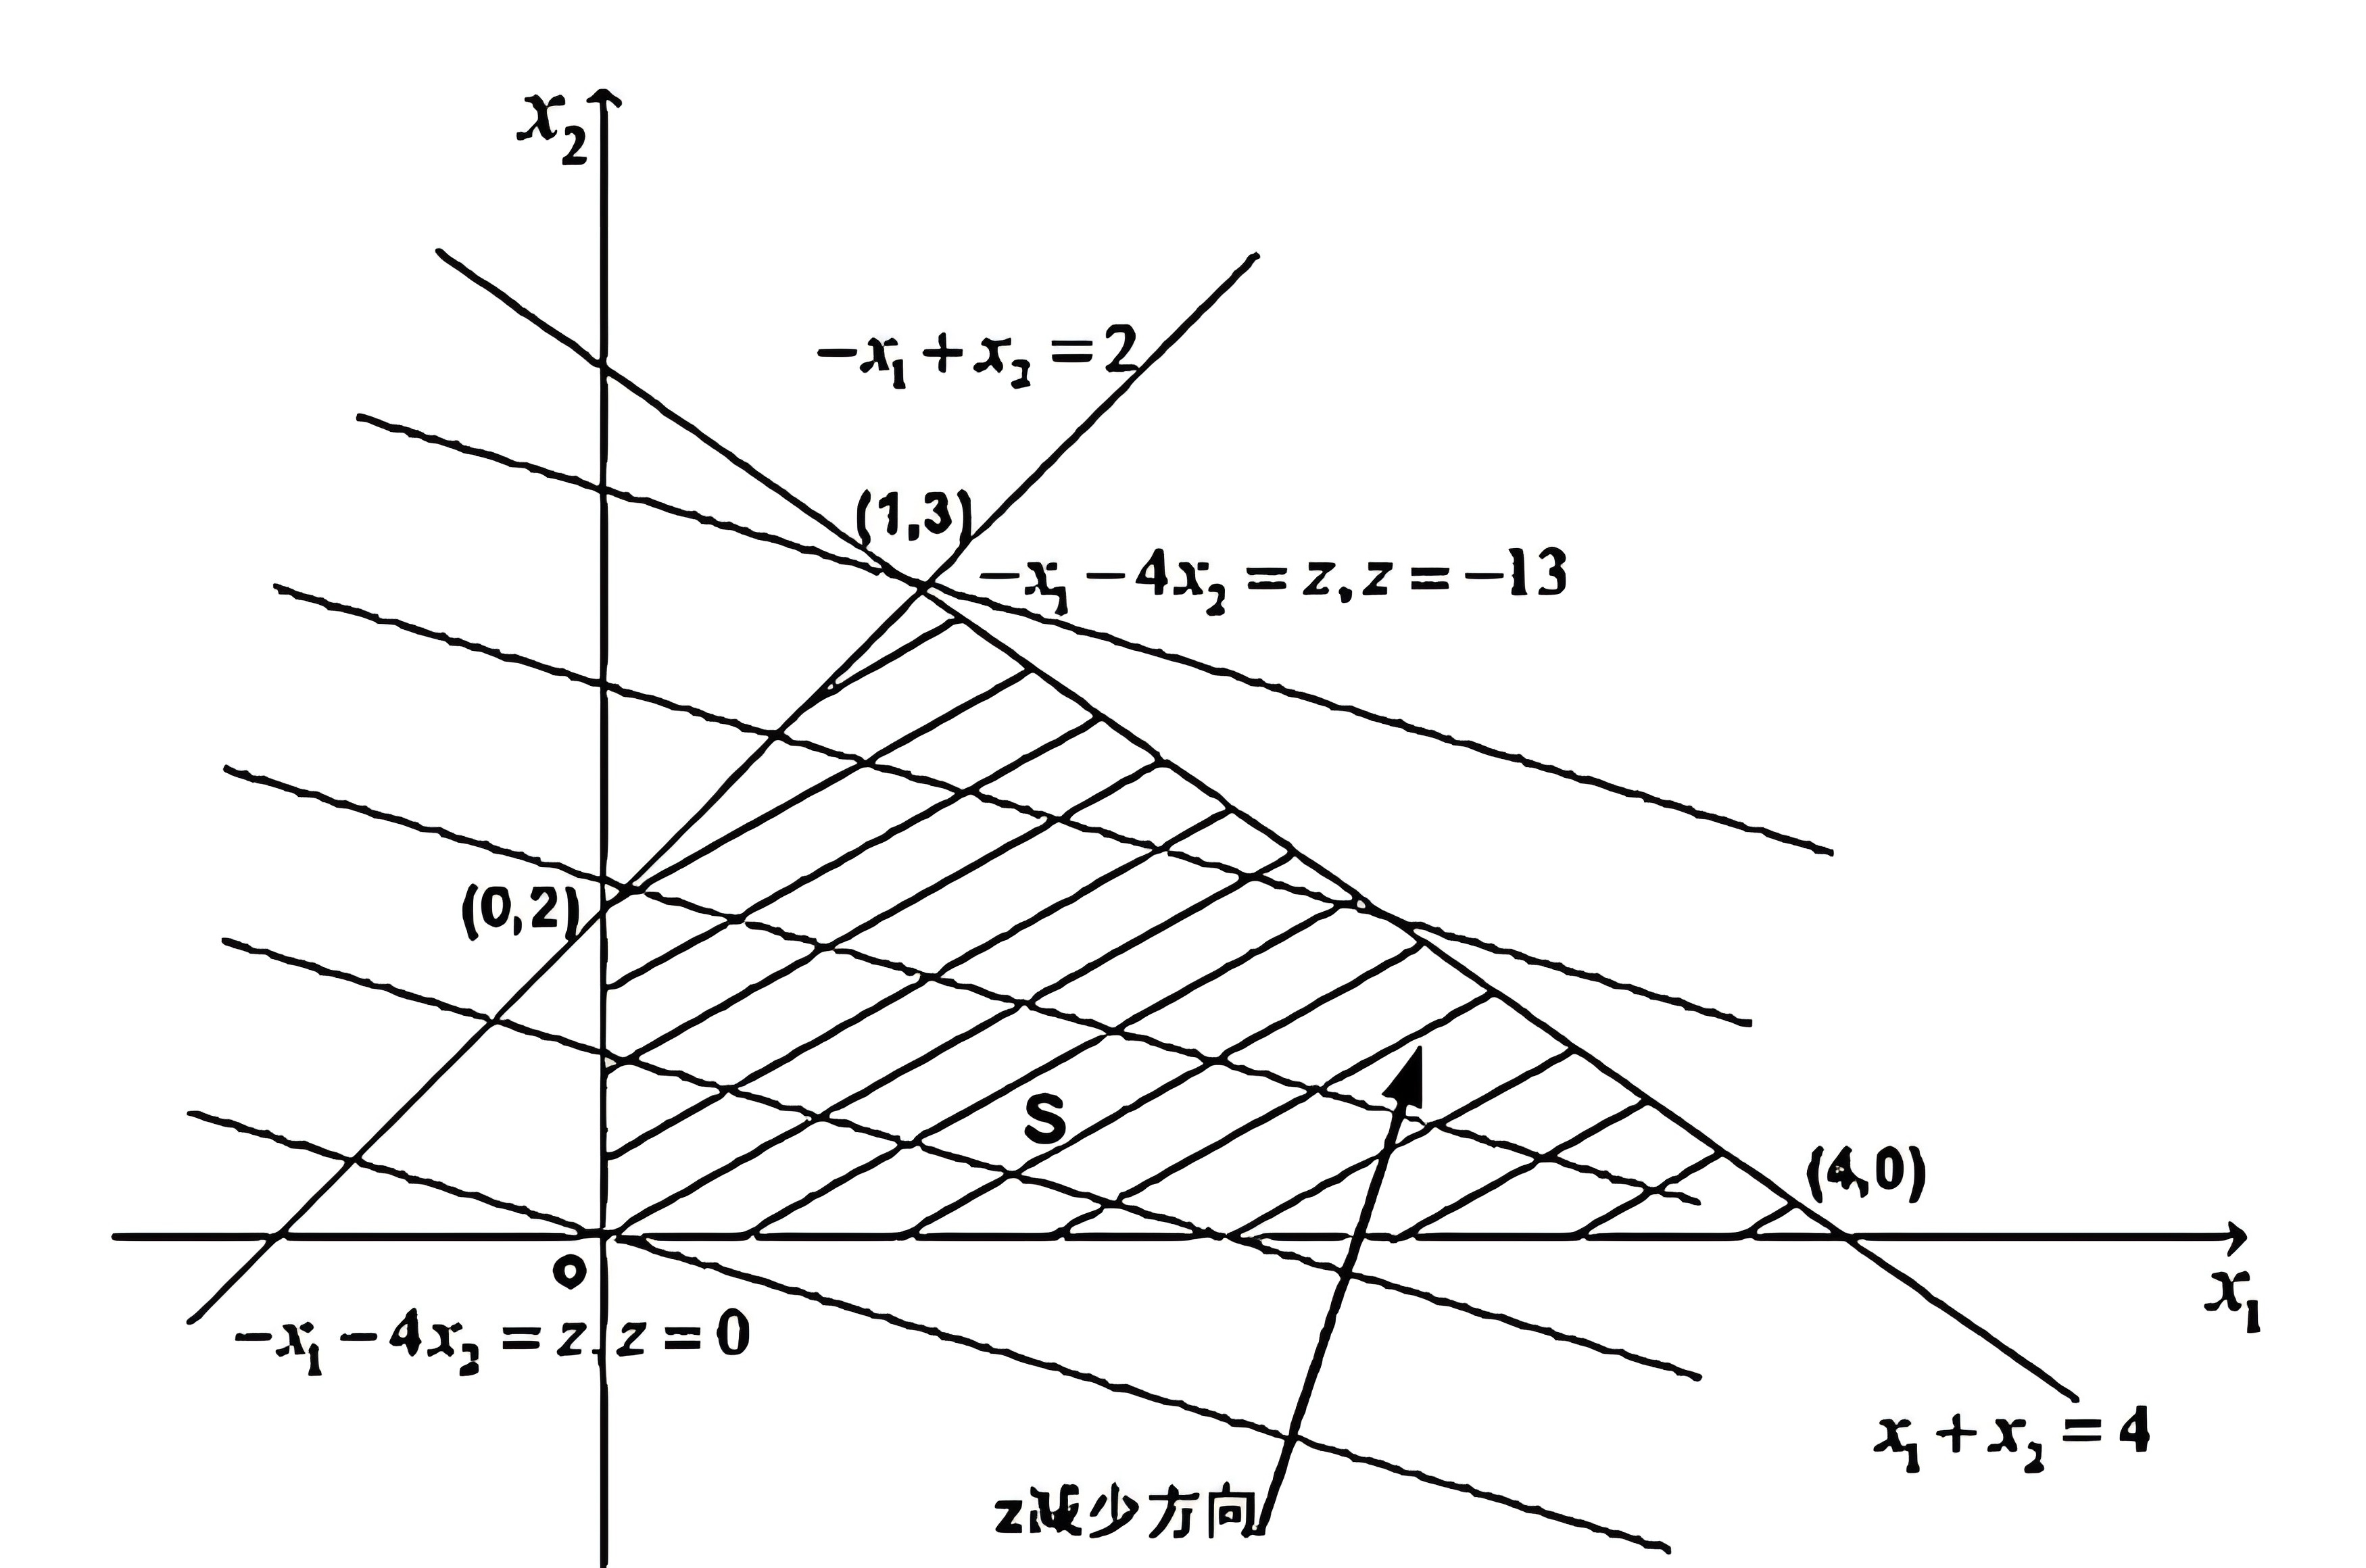
\includegraphics[width=0.6\textwidth]{./image/1.png}
        \caption{例1.1.3图解}
        \label{fig:Chapter2_Temporary_Pavilion_1}
    \end{figure}
    思考:
    \begin{itemize}
        \item \textbf{无穷多解}:上例中若取 $\min z = 3x_1 + 3x_2$ ,则目标函数线与 $x_2 + x_2 = 4$ 边界线重合,带来无穷多解。
        \begin{figure}[H]
            \centering
            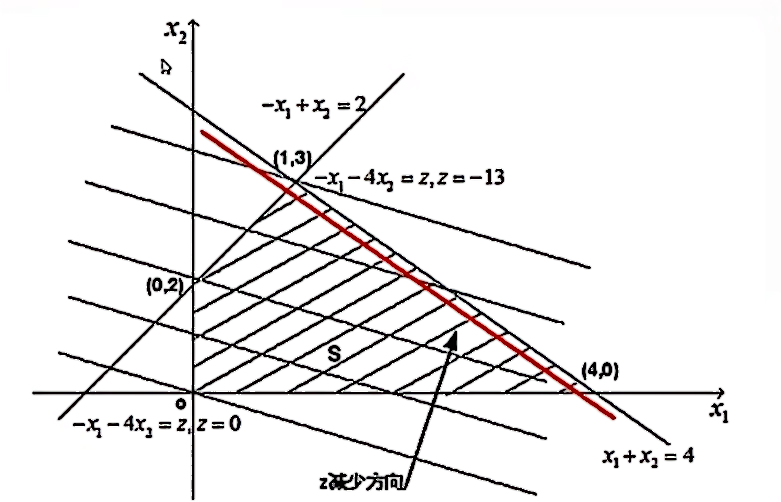
\includegraphics[width=0.4\textwidth]{./image/2.png}
            \label{fig:Chapter2_Temporary_Pavilion_2}
        \end{figure}
        \item \textbf{无界解}:例如下述线性规划问题:
        \begin{align*}
        \max z = x_1 &+ x_2 \\
        \text{s.t.} \quad  -2x_1 + x_2 & \leq 4 \\
         x_1 - x_2 & \leq 2 \\
         x_1, x_2 & \geq 0
        \end{align*}
        \begin{figure}[H]
            \centering
            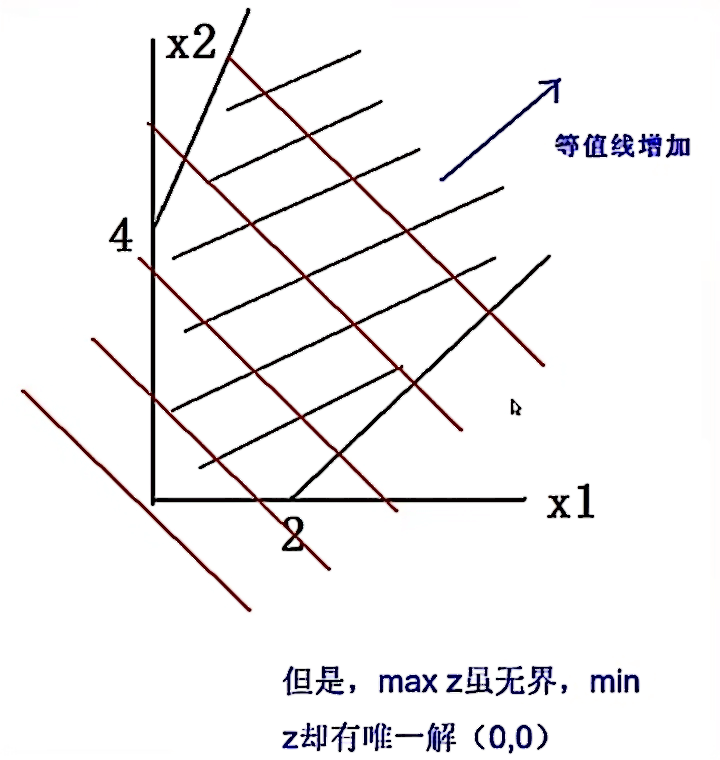
\includegraphics[width=0.4\textwidth]{./image/3.png}
            \label{fig:Chapter2_Temporary_Pavilion_3}
        \end{figure}
        \item \textbf{无最优解}:若可行域为空,则无可行解,自然无最优解。
    \end{itemize}


    \section{线性规划问题的数学模型}
    \begin{thmbox}{一般形式}{cool}
        特点:\textbf{目标函数}和\textbf{约束条件}都是决策变量的线性函数。
        \tcblower
        $\max(\min)\ z= \mathop{\sum}\limits_{j = 1}^{n}{c}_{j}{x}_{j}$

        s.t. $\begin{cases} \mathop{\sum }\limits_{j = 1}^{n}{a}_{ij}{x}_{j} \leq(\geq,=){b}_{i}\; & \left( {i = 1,2,\cdots ,m}\right) , \\  {x}_{j} \geq  0 & \left( {j = 1,2,\cdots ,n}\right) . \end{cases}$
        
        也可以表示为矩阵形式:
        
        $\max(\min)\ z = \mathbf{c}\cdot\mathbf{x}$

        s.t. $\begin{cases}\mathbf{A}\mathbf{x}\leq(\geq,=)\mathbf{b}, \\ \mathbf{x}\geq 0\end{cases}$\\
        其中称 $\mathbf{c} = \left( {{\mathrm{c}}_{1},{\mathrm{c}}_{2},\cdots ,{\mathrm{c}}_{\mathrm{n}}}\right)$ 为目标函数的\textbf{系数向量};\\
        称 $\mathbf{x} = {\left( {\mathrm{x}}_{1},{\mathrm{x}}_{2},\cdots ,{\mathrm{x}}_{\mathrm{n}}\right) }^{\mathrm{T}}$ 为\textbf{决策向量};\\
        称 $\mathbf{b} = \left( {{\mathrm{b}}_{1},{\mathrm{\;b}}_{2},\cdots ,{\mathrm{b}}_{\mathrm{m}}}\right)$ 了为约束方程组的\textbf{常数向量};\\
        称 $\mathbf{A} = {\left( {\mathrm{a}}_{\mathrm{{ij}}}\right) }_{\mathrm{m} \times  \mathrm{n}}$ 为约束方程组的\textbf{系数矩阵}; \\
        称 ${p}_{j} = {\left( {a}_{1j},{a}_{2j},\cdots ,{a}_{mj}\right) }^{T}$ 为约束方程组的\textbf{系数向量}.\\
    \end{thmbox}
    
    \begin{thmbox}{标准形}{cool}
        为了便于研究,规定线性规划模型的标准型。
        \tcblower
        $\max\ z = \mathbf{c}\cdot\mathbf{x}$

        s.t. $\begin{cases}\mathbf{A}\mathbf{x}=\mathbf{b}, \\ \mathbf{x}\geq 0\end{cases}$
    \end{thmbox}
    
    \begin{notebox}{\textbf{方法:一般形式化为标准形的方法}}
    \begin{itemize}[noitemsep]
        \item \textbf{目标函数}:若目标函数为$\min z$,则令$z'=-z$转化为$\max z'$。
        \item \textbf{约束条件}:若约束条件为不等式,可以再不等号左端加上/减去一个非负变量(称为\textbf{松弛变量})化为等式约束(哪边小,加哪边)。
        \item \textbf{决策变量}:若决策变量非正($x_j\leq 0$),则令$x_j'=-x_j$,$x_j'\geq 0$,转化为非负变量。
    \end{itemize}
    \end{notebox}

    \begin{exbox}{一般形式化标准形}{coolexample}
        \begin{align*}
            \min z = x_1 + 2x_2 &- 3x_3 \\
            x_1 + x_2 + x_3 &\leq 7 \\
            x_1 + x_2 + x_3 &\geq 2 \\
            - 3x_1 + x_2 + 2x_3 &= 5 \\
            x_1, x_2 &\geq 0
        \end{align*}
        化为标准形式。\\
        解:
        \begin{enumerate}
            \item 因 $x_3$ 无约束,令 $x_3 = x_4 - x_5,\;x_4,x_5\geq 0$
            \item $x_1 + x_2 + x_3 <  = 7 \rightarrow x_1 + x_2 + (x_4 - x_5) + \textcolor{red}{x_6} = 7$
            \item $x_1 + x_2 + x_3 >  = 2 \rightarrow x_1 + x_2 + (x_4 - x_5) = 2 + \textcolor{red}{x_7}$
            \item $- 3 x_1 + x_2 + 2 x_3 = 5 \rightarrow - 3 x_1 + x_2 + 2\left( {{x}_4 - {x}_5}\right) = 5$
            \\其中:$x_1,x_2,x_4,x_5,x_6,x_7>=0$
        \end{enumerate}
        此时再考虑目标函数

        $\min z=-x_1+2x_2-3x_3 \rightarrow \max z'=-z=x_1-2x_2+3x_4-3x_5+0x_6+0x_7$
    \end{exbox}

    \section{线性规划解的基本概念与基本理论}
    \label{2.3}
    \subsection{解}
    \begin{dfnbox}{可行解}{amznotes}
        满足Theorem 2.2.2约束条件的解$\mathbf{x}=(x_1,x_2,\cdots,x_n)^T$为线性规划问题的\textbf{可行解}。
    \end{dfnbox}
    \begin{dfnbox}{可行域}{amznotes}
        可行解全体构成的集合称为\textbf{可行域},记为$D$。
    \end{dfnbox}
    \begin{dfnbox}{最优解}{amznotes}
        使Theorem 2.2.2中目标函数达到最大的可行解称为\textbf{最优解}。
    \end{dfnbox}

    \subsection{基}
    \begin{dfnbox}{基}{amznotes}
        设系数矩阵 $A = {\left( {a}_{ij}\right) }_{m \times  n}$ 的秩为 $m$ ,则称 $A$ 的某个 $m \times  m$ 非奇
    异子矩阵 $B$ 为线性规划问题的一个\textbf{基}。
    \end{dfnbox}
    不妨设 $B = {\left( {a}_{y}\right) }_{m \times  m} = \left( {\mathbf{p}}_{1},{\mathbf{p}}_{2},\cdots ,{\mathbf{p}}_{m}\right)$
    \begin{itemize}
    \item \textbf{基向量}:向量 ${\mathbf{p}}_{j} = {\left( {a}_{1j},{a}_{2j},\cdots ,{a}_{mj}\right) }^{\mathrm{T}}\left( {j = 1,2,\cdots ,m}\right)$;
    \item \textbf{非基向量}:矩阵 $A$ 的其他列向量;
    \item \textbf{基变量}:与基向量对应的决策变量 ${\mathbf{x}}_{j}\left( j = 1,2,\cdots ,m \right)$;
    \item \textbf{非基变量}:其他的变量称为非基变量。
    \end{itemize}
    
    \subsection{基解}
    设问题的基为$B = \left( {\mathbf{p}}_{1},{\mathbf{p}}_{2},\cdots ,{\mathbf{p}}_{m}\right)$,将约束为:
    \begin{equation}
        \label{eq:2.1}
        \sum_{j=1}^{m} \mathbf{p}_{j}x_{j}=\mathbf{b} - \sum_{j=m+1}^{n} \mathbf{p}_{j}x_{j}
    \end{equation}
    \begin{dfnbox}{基解}{amznotes}
        在方程组 \hyperref[eq:2.1]{(2.1)} 的解中,令$x_j=0(j= m+1, m+2, \cdots , n)$,则解向量 
        \(\mathbf{x} = (x_{1}, x_{2}, \cdots, x_{m}, \cdots, 0, 0)\) 为问题的\textbf{基解}。
    \end{dfnbox}
    \begin{dfnbox}{基可行解、可行基}{amznotes}
        满足非负约束条件的基解称为\textbf{基可行解},对应于基可行解的基解为\textbf{可行基}。
    \end{dfnbox}

    \begin{notebox}{\textbf{方法:理解上述定义}}
        对于$A\mathbf{x}=\mathbf{b}$这样一个矩阵方程,我们以下面为例
        \[
            A = \begin{bmatrix}
            a_{11} & \textcolor{red}{a_{12}} & \textcolor{red}{a_{13}} & \textcolor{red}{a_{14}} & \textcolor{red}{a_{15}} & \textcolor{red}{a_{16}} & a_{17} \\
            a_{21} & \textcolor{red}{a_{22}} & \textcolor{red}{a_{23}} & \textcolor{red}{a_{24}} & \textcolor{red}{a_{25}} & \textcolor{red}{a_{26}} & a_{27} \\
            a_{31} & \textcolor{red}{a_{32}} & \textcolor{red}{a_{33}} & \textcolor{red}{a_{34}} & \textcolor{red}{a_{35}} & \textcolor{red}{a_{36}} & a_{37} \\
            a_{41} & \textcolor{red}{a_{42}} & \textcolor{red}{a_{43}} & \textcolor{red}{a_{44}} & \textcolor{red}{a_{45}} & \textcolor{red}{a_{46}} & a_{47} \\
            a_{51} & \textcolor{red}{a_{52}} & \textcolor{red}{a_{53}} & \textcolor{red}{a_{54}} & \textcolor{red}{a_{55}} & \textcolor{red}{a_{56}} & a_{57}
            \end{bmatrix}
            \quad
            \text{and}
            \quad
            \mathbf{x} =
            \begin{bmatrix}
            x_1 \\
            \textcolor{red}{x_2} \\
            \textcolor{red}{x_3} \\
            \textcolor{red}{x_4} \\
            \textcolor{red}{x_5} \\
            \textcolor{red}{x_6} \\
            x_7\\
            \end{bmatrix}
            \]
        观察,不难发现以下几个性质:
        \begin{itemize}
            \item $A$是一个$m \times n$的矩阵,其中$m<n$,这样决策变量才有多解;如果$m=n$即满秩,就只有唯一解了。
            \item 在矩阵$A$中选取一个$m \times m$的子矩阵$B$,并且这个子矩阵是非奇异的,那么就可以得到一个基,如标红所示。该子矩阵的m个行向量线性无关,m个列向量也线性无关。因此相当于一个m维空间中的坐标系。
            \item 基$B$中的每一个列向量就是基向量,不属于$B$但在$A$中的列向量就是非基向量。
            \item $A$右乘列向量$\mathbf{x}$,$\mathbf{x}$中标红的变量就是与基向量对应的决策变量,其他未标红的变量就是非基变量。
            \item 把基变量留下来,把非基变量移到等式右侧,令非基变量为0,得到的解就是基解;也就是将基$B$中的列向量与$\mathbf{x}$中的基变量相乘,得到的就是基解。换句话说,令$\mathbf{x}$中的非基变量为0,左乘$A$就可以得到基解;
            \item 如果基解本身均大于0,就是基可行解。
        \end{itemize}
    \end{notebox}
    \begin{dfnbox}{凸集}{amznotes}
        假设K为n维欧氏空间中的点集,如果对于任意两点,其连线上所有点均在K内,则称K为\textbf{凸集}。
    \end{dfnbox}
    例:实心圆、实心球是凸集,空心圆、空心球不是凸集。直观地说,凸集没有凹入部分。
    \begin{dfnbox}{凸集的顶点}{amznotes}
        对于凸集 $K$ 中的点 $x$,如果 $x$ 不能用相异的两点 $x^{(1)}, x^{(2)} \in K$ 的凸组合表示为
$x = \lambda x^{(1)} + (1 - \lambda) x^{(2)} \in K$ \quad $(0 \leq \lambda \leq 1)$。则称$x$为凸集K的一个顶点
    \end{dfnbox}
    对于凸集,顶点一般为边界点,但并非所有边界点都是顶点.
    

    \subsection{线性规划的几个重要定理}
    基于~\ref{2.3}节中代数学中求解方程和集合论的铺垫之后,我们可以得到几个z重要定理:
    \begin{thmbox}{定理}{cool}
        \begin{enumerate}
            \item 如果线性规划问题存在可行域 $D$,则其可行域 $D = \left\{ x \left| \; \sum_{j=1}^n \mathbf{p}_j x_j = \mathbf{b}, x_j \geq 0 \right. \right\}$ 一定是凸集。
            \item 线性规划问题(2.5),(2.6)的任一个基可行解$\mathbf{x}$必对应于可行域$D$的一个顶点。
            \item 对于可行域
            \begin{itemize}
                \item 如果可行域有界,则问题的最优解一定在可行域的顶点上达到。
                \item 如果可行域无界,则问题可能无最优解;若有最优解也一定在可行域的某个顶点上达到。
            \end{itemize}
        \end{enumerate}
    \end{thmbox}
        定理1的好处在于,凸集有很多良好的性质。

        定理2对我们求解没有太大帮助。

        定理3将求解最优化的可行域中无穷可解点的比较问题变成了三个定点的比较问题。
        \begin{figure}[H]
            \centering
            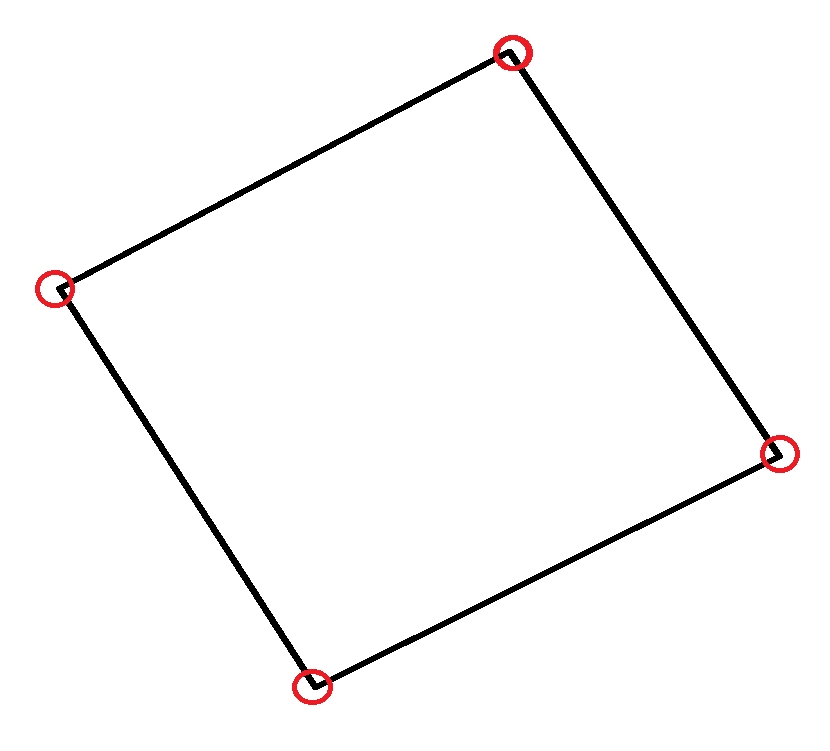
\includegraphics[width=0.6\textwidth]{./image/4.png}
            \caption{例如我们的可行域是上图中的这个四边形,最优解一定在这个四边形的四个顶点上,其他的可行域的点全都不必算。这样我们把无穷维(有无穷个点)的优化问题转化为有限的、可穷举的优化问题。}
            \label{fig:Chapter2_Temporary_Pavilion_4}
        \end{figure}
        总结来说,可以得到四个结论:
        \begin{enumerate}
            \item 线性规划所有可行解构成的集合为\textcolor{red}{凸集},也可能是\textcolor{red}{无界域};
            \item 线性规划的可行域有\textcolor{red}{有限}个顶点;
            \item 线性规划的每个基可行解对应可行域的\textcolor{red}{一个顶点};
            \item 若线性规划有最优解,必定在\textcolor{red}{某个顶点}上达到,但\textbf{并非只能在顶点上达到}。\\
            (比如一个函数在某处有最大值,不是说只有在这一处能达到最大值,可能$f(x_1)=f(x_2)=f_{max},x_1\neq x_2$)
        \end{enumerate}
        本质上可以理解为\textbf{一个可行域内的点,只有顶点是线性无关的,其他任何点都可以由顶点线性表示}。\\
        这些结论构成了单纯形法的理论基础。
    \section{线性规划求解的单纯形法}
    \label{2.4}
    \begin{notebox}{求解线性规划问题的方法}
        \begin{enumerate}
            \item 求一个基可行解(即对应可行域的一个顶点);
            \item 检查该基可行解是否为最优解;
            \begin{itemize}
                \item 如果不是,则设法再求另一个没有检查过的基可行解(可行域内另一个顶点),如此进行下去,直到得到某一个基可行解为最优解为止;
                \item 如果是,结束。
            \end{itemize}
        \end{enumerate}
    \end{notebox}
    这个过程本质上就是先找到可行域内任意一个顶点,然后跳到其他顶点上,穷举的办法求谁最大。就好像我们在函数中,有许多极大值,但是要都求出来去求最大值。
    如果用函数来类比,~\ref{2.4.1}中所做的就是先找到任意一个极大值点$x_1$,~\ref{2.4.2}中所做的就是利用$x_1$便捷地去找其他极大值点;
    \\那么我们不禁要问:
    \begin{itemize}
        \item 如何求出第一个基可行解?(如何找到$x_1$?)
        \item 如何由一个基可行解过渡到另一个基可行解?(怎么通过$x_1$快速找到其他极大值点?)
        \item 如何判断基可行解是否为最优解?(哪个极大值点是最大值点?)
    \end{itemize}
    解决这些问题的方法称为\textbf{单纯形法}。
    \subsection{初始基可行解的确定}
    \label{2.4.1}
    \begin{notebox}{\textbf{初始基可行解的确定方法}}
        \begin{enumerate}
            \item \textbf{标准化}:第一步,将线性规划模型化为标准型;
            \item \textbf{解方程}:第二步,解矩阵方程,得到基可行解。
        \end{enumerate}
    \end{notebox}
    这一步骤本质上是\textbf{找到可行域的任意一个顶点},且只能硬着头皮算。考虑到读者可能和笔者一样忘记了线性代数的相关内容,因此在这里对矩阵方程解法加以补充:
    现在假设我们有:
    \[
    \quad
    A = \begin{bmatrix}
    1 & 2 & 3 & 4 & 5 \\
    2 & 3 & 4 & 5 & 6 \\
    3 & 4 & 5 & 6 & 7
    \end{bmatrix}, \quad
    \mathbf{x} = \begin{bmatrix}
    x_1 \\
    x_2 \\
    x_3 \\
    s_1 \\
    s_2
    \end{bmatrix}, \quad
    \mathbf{b} = \begin{bmatrix}
    4 \\
    5 \\
    7
    \end{bmatrix}
    \] 
    \begin{itemize}
        \item 从系数矩阵 $A = \left( a_{ij} \right)_{m \times n}$
        $\left( m < n, \text{秩为} m \right)$ 总可以得到一个 $m$ 阶单位阵 $E_{m}$ 。(例如,可以通过  
        高斯消元法对系数矩阵 $A$ 进行行初等变换,得到一个 $m$ 阶单位阵 $E_{m}$ )。  
        $A\mathrm{x} = \mathrm{b} \rightarrow \left[ E_{m} \text{ 其他元素} \right] \mathrm{x'} = \mathrm{b'}$.\\

        \[
        A \xrightarrow{\text{初等变换}} \begin{bmatrix}
        \textcolor{red}{1} & \textcolor{red}{0} & \textcolor{red}{0} & -2 & -3 \\
        \textcolor{red}{0} & \textcolor{red}{1} & \textcolor{red}{0} & -3 & -4 \\
        \textcolor{red}{0} & \textcolor{red}{0} & \textcolor{red}{1} & 0 & 0
        \end{bmatrix}
        \]

        \item 取如上 $m$ 阶单位阵 $E_{m}$ 为初始可行基,即 $B = E_{m}$, 将相应的约束方程组变为:
        ${x}_i = {b}_i - {a}_{i,m + 1}{x}_{m + 1} - \cdots - {a}_{i,n}{x}_n \quad (i = 1, 2, \cdots, m)$.  
        \\
        \[
        \begin{bmatrix}
        \textcolor{red}{1} & \textcolor{red}{0} & \textcolor{red}{0} & -2 & -3 \\
        \textcolor{red}{0} & \textcolor{red}{1} & \textcolor{red}{0} & -3 & -4 \\
        \textcolor{red}{0} & \textcolor{red}{0} & \textcolor{red}{1} & 0 & 0
        \end{bmatrix}
        \times
        \begin{bmatrix}
        \textcolor{red}{x_1} \\
        \textcolor{red}{x_2} \\
        \textcolor{red}{x_3} \\
        \textcolor{blue}{s_1} \\
        \textcolor{blue}{s_2}
        \end{bmatrix}
        =
        \begin{bmatrix}
        4 \\
        5 \\
        7
        \end{bmatrix}
        \]

        \[
        \text{解得列向量:}
        \quad \begin{bmatrix}
        4 \\
        5 \\
        7 \\
        0 \\
        0
        \end{bmatrix}
        \]

        \item 令方程组后面的 $n - m$ 个变量为 0, ${x}_j = 0 \quad (j = m + 1, m + 2, \ldots, n)$,
        则可得一个初始基可行解: 
        ${x}^{(0)} = \left( {x}_1^{(0)}, {x}_2^{(0)}, \ldots, {x}_m^{(0)}, 0, \ldots, 0 \right)^T = \left( {b}_1, {b}_2, \cdots, {b}_m, 0, \cdots, 0 \right)^T$.\\
        \[
        \text{令非基变量为0:}
        \quad \begin{bmatrix}
        4 \\
        5 \\
        7 \\
        0 \\
        0
        \end{bmatrix}
        \]
    \end{itemize}

    \subsection{寻找另一个基可行解:基变换法}
    \label{2.4.2}
    为了确定在其他顶点上的可行解,我们需要使用\textbf{基变换法}的方法。
    \begin{notebox}{\textbf{基变换法}}    
    \\当一个基可行解不是最优解或不能判断时,需要过渡到另一个基可行解,即从基可行解,
    \[
    \mathbf{x}^{(0)} = \left( x_1^{(0)}, x_2^{(0)}, \ldots, x_m^{(0)}, 0, \ldots, 0 \right)^T
    \]
    对应的可行基 

    \[
    B = \left( p_1, p_2, \ldots, p_m \right)
    \]
    中替换一个列向量,用来替换的列向量与原向量组未被替换的向量线性无关。

    例如,用非基变量 \( p_{m+t} \left( 1 \leq t \leq n - m \right) \) (称为换入变量)替换基变量 \( p_1 \left( 1 \leq 1 \leq m \right) \) (称为换出变量),就可得到一个新的可行基

    \[
    B_1 = \left( p_1, \ldots, p_{1-1}, p_{m+t}, p_{1+1}, \ldots, p_m \right)
    \]
    从而可以求出一个新的基可行解

    \[
    \mathbf{x}^{(1)} = \left( x_1^{(1)}, x_2^{(1)}, \ldots, x_m^{(1)}, 0, \ldots, 0 \right)^T
    \]
    \end{notebox}
    我们仍然用刚才的例子:

    \[
    A' = \begin{bmatrix}
    1 & 0 & 0 & -2 & -3 \\
    0 & 1 & 0 & -3 & -4 \\
    0 & 0 & 1 & 0 & 0
    \end{bmatrix}
    \]
    这是初始变换后的矩阵 \( A' \),前三列已经是单位矩阵。

    % 步骤 1:交换第三列和第四列后的矩阵 A''

    \[
    A'' = \begin{bmatrix}
    1 & 0 & \textcolor{pink}{0} & \textcolor{blue}{-2} & -3 \\
    0 & 1 & \textcolor{pink}{0} & \textcolor{blue}{-3} & -4 \\
    0 & 0 & \textcolor{pink}{1} & \textcolor{blue}{0} & 0
    \end{bmatrix}
    \]
    在这个步骤中,我们交换了 \( A' \) 的第三列和第四列,粉色为换出变量,蓝色为换入变量。

    % 步骤 2:经过初等变换后的矩阵 A'''

    \[
    A''' = \begin{bmatrix}
    1 & 0 & 0 & * & * \\
    0 & 1 & 0 & * & * \\
    0 & 0 & 1 & * & *
    \end{bmatrix}
    \]
通过适当的初等变换(例如对第三列和第四列进行适当的线性组合),我们将前三列转换为单位矩阵,最终得到了这个矩阵。这样我们得到了一个新的可行基,以此可以继续解方程得到另一个可行解。\\
当然,也有可能换入非基变量后,我们应该首先检查更换后的“基”是否可逆,比如发现新的三个列向量线性相关而不是线性无关,不能构成一个基,那么此时应该换一个非基变量换入。
\begin{thmbox}{线性规划模型的另一个基可行解}{cool}
    事实上,这个新的基可行解可以用以下公式直接计算出来:
    \[
    \mathbf{x}_i^{(1)} = \left\{
    \begin{matrix}
    \mathbf{x}_i^{(0)} - \theta \beta_{i, m+t}, & i \neq l \\
    \theta, & i = l
    \end{matrix}
    \right.
    \quad
    \left( \begin{matrix}
    i = 1, 2, \cdots, m, \\
    1 \leq l \leq m, 1 \leq t \leq n - m
    \end{matrix} \right)
    \]
    其中
    \[
    \theta = \frac{\mathbf{x}_i^{(0)}}{\beta_{i, m+t}} = \min\limits_{1 \leq i \leq m} \left\{ \frac{\mathbf{x}_i^{(0)}}{\beta_{i, m+t}} \mid \beta_{i, m+t} > 0 \right\},
    \]
    并且
    \[
    \mathbf{p}_{m+t} = \sum\limits_{i=1}^{m} \beta_{i, m+t} \mathbf{p}_i.
    \]
    如果 \( \mathbf{x}^{(1)} = \left( \mathbf{x}_1^{(1)}, \mathbf{x}_2^{(1)}, \ldots, \mathbf{x}_m^{(1)}, 0, \ldots, 0 \right)^T \) 仍不是最优解,则可以重复利用这种方法,直到得到最优解为止。
\end{thmbox}
    \subsection{最优性检验方法}
    实际上,我们并不需要把所有的“顶点”都找到再去比较哪个最大。我们可以找到可行域中的\textbf{任意一点},因为这个点是不独立的(可以由其他所有顶点线性表示),
    所以如果我们找到了一个顶点$x_1$,得到目标函数值$z_1=cx_1$;而有任一点$x=a_1x_1+a_2x_2+\cdots+a_nx_n$,
    得到目标函数值$z=cx$。只需要比较$z_1$和$z$,即可知道$z_1$是否是最大值,证明过程如下(感兴趣的同学可以了解):\\
    将基可行解 \( \mathbf{x}^{(1)} \) 和这个任意的 \( \mathbf{x} = \left( x_1, x_2, \ldots, x_n \right)^T \) 分别代入目标函数得:
    \[
    z^{(1)} = \sum_{i=1}^{m} c_i x_i^{(1)} = \sum_{i=1}^{m} c_i b_i^{\prime}, \psi
    \]

    \[
    z = \sum_{i=1}^{n} c_i x_i = \sum_{i=1}^{m} c_i x_i + \sum_{i=m+1}^{n} c_i x_i
    \]

    \[
    = \sum_{i=1}^{m} c_i \left( b_i^{\prime} - \sum_{j=m+1}^{n} a_{ij}^{\prime} x_j \right) + \sum_{j=m+1}^{n} j j^+ j
    \]

    \[
    = \sum_{i=1}^{m} c_i b_i^{\prime} + \sum_{j=m+1}^{n} \left( c_j - \sum_{i=1}^{m} c_i a_{ij}^{\prime} \right) x_j^{\prime}
    \]

    \[
    = z^{(1)} + \textcolor{red}{\sum_{j=m+1}^{n} \left( c_j - z_j \right) x_j}
    \]

    其中 \( z_j = \sum_{i=1}^{m} c_i a_{ij}^{\prime} \quad (j = m+1, \cdots, n) \)。 记 \( \sigma_j = c_j - z_j \quad (j = m+1, \cdots, n) \),则

    \[
    z = z^{(1)} + \textcolor{red}{\sum_{j=m+1}^{n} O_j x_j} \quad \
    \]
    注意到:
    当 \( \sigma_j > 0 \quad (j = m+1, \cdots, n) \) 时,就有

    \[
    z > z^{(1)} ;
    \]
    当 \( \sigma_j \leq 0 \quad (j = m+1, \cdots, n) \) 时,就有

    \[
    z \leq z^{(1)}.
    \]

    为此,\( \sigma_j = c_j - z_j \) 的符号是判别 \( \mathbf{x}^{(1)} \) 是否为最优解的关键所在,故称之为\textcolor{red}{检验数}。于是可以得出下面的结论:
    \begin{notebox}{\textbf{判断最优解的办法}}
        \begin{enumerate}
            \item 如果 \( \sigma_j \leq 0 \quad (j = m+1, \cdots, n) \),则 \( \mathbf{x}^{(1)} \) 是问题的最优解,最优值为 \( z^{(1)} \);
            \item 如果 \( \sigma_j \leq 0 \quad (j = m+1, \cdots, n) \),且至少存在一个 \( \sigma_{m+k} = 0 \quad (0 \leq k \leq n-m) \),
            则问题有无穷多个最优解,\( \mathbf{x}^{(1)} \) 是其中之一,最优值为 \( z^{(1)} \);
            \item 如果 \( \sigma_j < 0 \quad (j = m+1, \cdots, n) \),则 \( \mathbf{x}^{(1)} \) 是问题的唯一最优解,最优值为 \( z^{(1)} \);
            \item 如果存在某个检验数 \( \sigma_{m+k} > 0 \quad (0 \leq k \leq n-m) \),并且对应的系数向量 \( \mathbf{p}_{m+k} \) 的各分量
            \( a_{i, m+k} \leq 0 \quad (i = 1, 2, \cdots, m) \),则问题具有无界解(即无最优解)。
        \end{enumerate}
    \end{notebox}
    
    ~\ref{2.4}\textbf{节所有上述所有过程一般上不需要我们了解的过于深入,因为有现成的计算机函数可以用,但是可以领会其思想。}


    \section{线性规划问题的灵敏度分析}
    在线性规划模型
    \[
    \max z = \mathbf{c} \cdot \mathbf{x}
    \]
    约束条件为

    \[
    \left\{
    \begin{array}{l}
    \mathbf{A} \mathbf{x} = \mathbf{b} \\
    \mathbf{x} \geq \mathbf{0}
    \end{array}
    \right.
    \]
    其中,总假设 \( \mathbf{A}, \mathbf{b}, \mathbf{c} \) 都是常数,但这些数值在许多情况下是由试验或测量得到的,特别是在迭代计算中,这些数值都是近似值。通常,\( \mathbf{A} \) 表示工艺条件,\( \mathbf{b} \) 表示资源条件,\( \mathbf{c} \) 表示市场条件。在实际中,可能有多种原因引起它们的变化。

    现在的问题是:这些系数在什么范围内变化时,线性规划问题的最优解不发生变化?这就是灵敏度分析要研究的问题。\\
    \textbf{这一问题比较复杂,本课程不做深入探究,但是大作业可以考虑}



    \section{应用案例分析}
    \subsection{下料问题}
    \begin{exbox}{下料问题}{coolexample}
        某单位需要加工作 100 套工架,每套工架需用长为 2.9m,2.1m 和1.5m 的圆钢各一根,已知原材料长 7.4m,现在的问题是如何下料使得所用的原材料最省?

        解:
        简单分析,在每一根原材料上各截取一根 2.9m,2.1m 和 1.5m的圆钢做成一套工架,每根原材料剩下料头 0.9m。要完成 100 套工架,就需要用 100 根原材料,共剩余 90m 料头。
        \\若采用套截方案,则可以节省原材料。下面给出了几种可能的套截方案,如表2.1所示。\\
        实际上,为了保证完成这100套工架,使所用原材料最省,可以混合使用各种下料方案。\\
        设按方案 \( A, B, C, D, E \) 下料的原材料数分别为 \( x_1, x_2, x_3, x_4, x_5 \)。根据表格 2-1,可以得到如下线性规划模型。
        目标函数:

        \[
        \min z = 0x_1 + 0.1x_2 + 0.2x_3 + 0.3x_4 + 0.8x_5
        \]

        约束条件:

        \[
        \begin{cases}
        x_1 + 2x_2 + x_4 = 100 \\
        2x_3 + 2x_4 + x_5 = 100 \\
        3x_1 + x_2 + 2x_3 + 3x_5 = 100 \\
        x_1, x_2, x_3, x_4, x_5 \geq 0
        \end{cases}
        \]
        所有 \( 2.9 \) 的料总数 100,所有 \( 2.1 \) 的料总数 100,所有 \( 1.5 \) 的料总数 100。
    \end{exbox}

    \begin{table}[H]  % 使用 H 强制放置位置
        \centering
        \renewcommand{\arraystretch}{1.5} % 调整行高
        \begin{tabular}{|c|c|c|c|c|c|}
        \hline
        \multirow{2}{*}{长度/m} & \multicolumn{5}{c|}{方案} \\ \cline{2-6} 
         & A & B & C & D & E \\ \hline
        2.9 & 1 & 2 & 0 & 1 & 0 \\ \hline
        2.1 & 0 & 0 & 2 & 2 & 1 \\ \hline
        1.5 & 3 & 1 & 2 & 0 & 3 \\ \hline
        合计/m & 7.4 & 7.3 & 7.2 & 7.1 & 6.6 \\ \hline
        料头/m & 0 & 0.1 & 0.2 & 0.3 & 0.8 \\ \hline
        \end{tabular}
        \caption{例2.6.1下料方案}
    \end{table}
        
        \begin{codebox}{MATLAB代码}{线性规划求解}
            \begin{amzcode}{matlab}
                c = [0, 0.1, 0.2, 0.3, 0.8]';
                b1 = [0, 0, 0, 0, 0]';
                b2 = [100, 100, 100]';
                A1 = [-1, 0, 0, 0, 0; 0, -1, 0, 0, 0; 0, 0, -1, 0, 0; 0, 0, 0, -1, 0; 0, 0, 0, 0, -1]';
                A2 = [1, 2, 0, 1, 0; 0, 0, 2, 2, 1; 3, 1, 2, 0, 3]';
                [x, fv] = linprog(c, A1, b1, A2, b2);
            \end{amzcode}
        \end{codebox}
        
        运行该程序后,立即可以得到最优解为 $\mathbf{x}=(12.8243\text{,}27.1757\text{,}17.1757\text{,}32.8243\text{,}0)^{\mathrm{T}}$。四舍五入的方法取整得
        $\mathbf{x}=(13,27\text{,}17\text{,}33\text{,}0)^{\mathrm{T}}$。最优值为$z=16$,即接方案 A 下料 13 根,方案B下料 27 根,方案 c下料 17 根,方案 D 下料 33 根,共需原材料 90 根就可以制作完成 100 套工架,剩余料头最少为 16m。

        \begin{notebox}{\textbf{matlab代码解析}}
            \begin{enumerate}
                \item \textbf{目标函数定义}:\\
                \texttt{c = [0, 0.1, 0.2, 0.3, 0.8]'} 定义了最小化料头长度的目标函数系数向量,对应五种下料方案的料头长度。
            
                \item \textbf{约束条件设置}:
                \begin{itemize}
                    \item \texttt{b1 = [0, 0, 0, 0, 0]'} 设置变量非负约束的右端项
                    \item \texttt{b2 = [100, 100, 100]'} 设置三种圆钢需求量的右端项
                    \item \texttt{A1} 矩阵通过负单位矩阵实现 $x_i \geq 0$ 的非负约束
                    \item \texttt{A2} 矩阵的每一列对应一个下料方案:
                    \begin{itemize}
                        \item 第一行:2.9m圆钢的生产数量约束
                        \item 第二行:2.1m圆钢的生产数量约束
                        \item 第三行:1.5m圆钢的生产数量约束
                    \end{itemize}
                \end{itemize}
            
                \item \textbf{线性规划求解}:\\
                \texttt{linprog(c, A1, b1, A2, b2)} 调用MATLAB线性规划求解器,其中:
                \begin{itemize}
                    \item 输入参数:目标系数 \texttt{c},不等式约束 \texttt{A1, b1},等式约束 \texttt{A2, b2}
                    \item 输出参数:\texttt{x} 为最优解向量,\texttt{fv} 为最优目标值
                \end{itemize}
            
                \item \textbf{结果修正}:\\
                原始解包含小数,通过四舍五入得到整数解 \texttt{(13,27,17,33,0)},此时总用料90根,剩余料头16m。
            \end{enumerate}
        \end{notebox}
        
        
        \begin{codebox}{LINGO代码}{线性规划模型}
            \begin{amzcode}{matlab}
                MODEL
                sets;
                row/1 2 3/:b;
                arrange/1..5/:x c;
                endsets;

                data:
                b=100,100,100;
                c=0 0 1 0.2 0 3 0.8.
                a=1,2,0,1,0,0,0,2,2,1 3,1 2,0,3;
                enddata.

                [oBJ] min=@sum(arrange(j):c(j)*x(j));
                @for(row(i):@sum(arrange(j);a(lj)*x(j))=b(i););
                @for(arrange(j);x(j)>=0;);
                END
            \end{amzcode}
        \end{codebox}
        
        运行该程序后,立即可以得到最优解为 $\mathbf{x}=(0\text{,}40\text{,}30\text{,}20\text{,}0)^{\mathrm{T}}$,最优值为 $z=16$,即按方案 B下料 40 根,方案C下料 30 根,方案 D 下料 20 根,共需原材料 90根就可以制作完成 100 套工架,剩余料头最少为 16m。

        \subsection{连续投资问题}
        
        \begin{exbox}{连续投资问题}{coolexample}
            某投资公司拟制定今后5年的投资计划,初步考虑下面的四个投资项目:
            \\项目A:从第1年到第4年每年年初需要投资,于次年年末收回成本,并可获利润 15\%;。
            \\项目 B:第3年年初需要投资.到第5年年末可以收回成本,并获得利润 25\%但为了保证足够的资金流动,规定该项目的投资金额上限为不超过总金额的40%;
            \\项目C:第2年年初需要投资,到第5年年来可以收回成本,并获得利润 40\%,
            但规定该项目的最大投资金额不超过总金额的 30\%;
            \\项目D:5年内每年年初可以购买公债,于当年年末可以归还本金,并获利息 6\%。
            \\该公司现有投资金额 100万元,请你帮助该公司制定这些项目每年的投资计划,使公司到第5年年末能够获得最大的利润。
            \\
            \\
            解:
            虽然这是一个连续投资问题,即属于动态优化问题,但是在这里可以用静态优化的方法来解决。用决策变量分别表示第i年年初为项目 A,B,C,D的投资额,根据问题的要求各变量的对应关系如表2-7所示(表格待补充),表中空白处表示当年不能为该项目投资,也可认为投资额为0。\\
            \\
            首先注意到,项目 \(D\) 每年都可以投资,并且当年末就能收回本息,所以公司每年应把全部资金都投出去。因此,投资方案应满足下面的条件。
            第 1 年:将 100 万元资金全部用于项目 \(A\) 和项目 \(D\) 的投资,即:

            \[
            x_{11} + x_{14} = 1000000
            \]
            第 2 年:因为第 1 年用于项目 \(A\) 的投资到第 2 年年末才能收回,所以能用于第 2 年年初的投资金额只有项目 \(D\) 的第 1 年收回的本息总额 \(x_{14}(1 + 0.06)\)。于是第 2 年的投资分配为:

            \[
            x_{21} + x_{23} + x_{24} = 1.06 x_{14}
            \]

            于是可以得到问题的线性规划模型为:

            \[
            \max z = 1.15 x_{41} + 1.25 x_{32} + 1.40 x_{23} + 1.06 x_{54}
            \]
            约束条件如下:

            \[
            \begin{aligned}
            x_{11} + x_{14} &= 1000000 \\
            -1.06 x_{14} + x_{21} &+ x_{23} + x_{24} = 0 \\
            -1.15 x_{11} - 1.06 x_{24} &+ x_{31} + x_{32} + x_{34} = 0 \\
            -1.15 x_{21} - 1.06 x_{34} &+ x_{41} + x_{44} = 0 \\
            -1.15 x_{31} - 1.06  &x_{44} + x_{54} = 0 \\
            x_{32} \leq &400000 \\
            x_{32} \leq &300000 \\
            x_{33} \leq x_{33} &+ x_{44} \leq 0.3 \\
            4 \leq &t \leq 5
            \end{aligned}
            \]
            考虑到这个问题的实际情况,这里使用 LINGO 求解该线性规划模型。

            运行该程序后,得到最优解:

            $
            x_{11} = 716981.1
            ,
            x_{14} = 283018.9
            ,
            x_{23} = 300000
            ,
            x_{31} = 424528.3
            ,
            x_{32} = 400000
            ,
            x_{54} = 488207.5
            $
            
            其他的变量均为零,最优值为:

            \[
            z = 1437500
            \]
            即连续投资方案为:
            \begin{itemize}
                \item 第 1 年用于投资项目 \(A\) 的金额为 716981.1 元,项目 \(D\) 的金额为 283018.9 元。
                \item 第 2 年用于项目 \(C\) 的投资金额为 300000 元。
                \item 第 3 年用于项目 \(A\) 的投资为 424528.3 元,项目 \(B\) 的金额为 400000 元。
                \item 第 5 年用于投资项目 \(D\) 的金额为 488207.5 元。
            \end{itemize}
            到第 5 年年末,该公司拥有总资金为 1437500 元,收益率为 43.75\%。
            \end{exbox}

            
\ifx\allfiles\undefined
	
	% 如果有这一部分的参考文献的话,在这里加上
	% 没有的话不需要
	% 因此各个部分的参考文献可以分开放置
	% 也可以统一放在主文件末尾。
	
	%  bibfile.bib是放置参考文献的文件,可以用zotero导出。
	% \bibliography{bibfile}
	
	end{document}
	\else
	\fi